\section{Introduction}

Collecting detailed information about wild animals~\cite{Prangle2006NewRadiocolars,Rutz2012AutomatedMapping} 
remains a significant technical challenge that
limits the ability of ecologists to study the interactions between wildlife and their environment. 
One tool that emerged a little over a decade ago
and has been gaining significance is 
{\em encounter detection and logging}~\cite{Tentelier2016FishNetwork,
Bohm2009WildlifeLivestock,Ripperger2016ProximitySensing}.

Encounter-registration system~\cite{Levin2015Performance,Menhill2012NovelTelemetry,dressler2016bats} 
is a kind of wildlife tracing systems,
consisting of radio devices called {\em tags} attached to wild
animals (and sometimes also to fixed positions and livestock), as depicted in Fig.~\ref{tags}. 
The radios transmit identification
packets periodically and listen to such packets from other tags,
recording data about received packets in persistent memory in the tag. The
radios are typically configured for short-range communication by using low transmitting power and by 
using high data-rates (both limit the signal-to-noise ratio at the receiver). Since the radios
are configured for short-range communication, receiving a packet implies the transmitting tag is
in close proximity to the receiving tag. Recent systems record each packet with received signal strength
indication (RSSI)~\cite{Daiya2011Experimental}, helping to estimate the distance between the transmitter and receiver.
This is the main goal of these systems: to log close-proximity
events between two or more animals. The logs are downloaded either by physically retrieving the tags,
or by remotely downloading to base-stations placed in locations that the animals pass by frequently.

Such systems have gained popularity among ecologists because 
the tags are relatively inexpensive and can
be very small. In addition, their deployment does not require much infrastructure in the field.
More importantly, these systems help to study the close-proximity encounters of wildlife, 
which are key aspects of many significant 
events in the life of animals: mating, predation, disseminating diseases, etc.


\begin{figure}[!t]
    \centering
    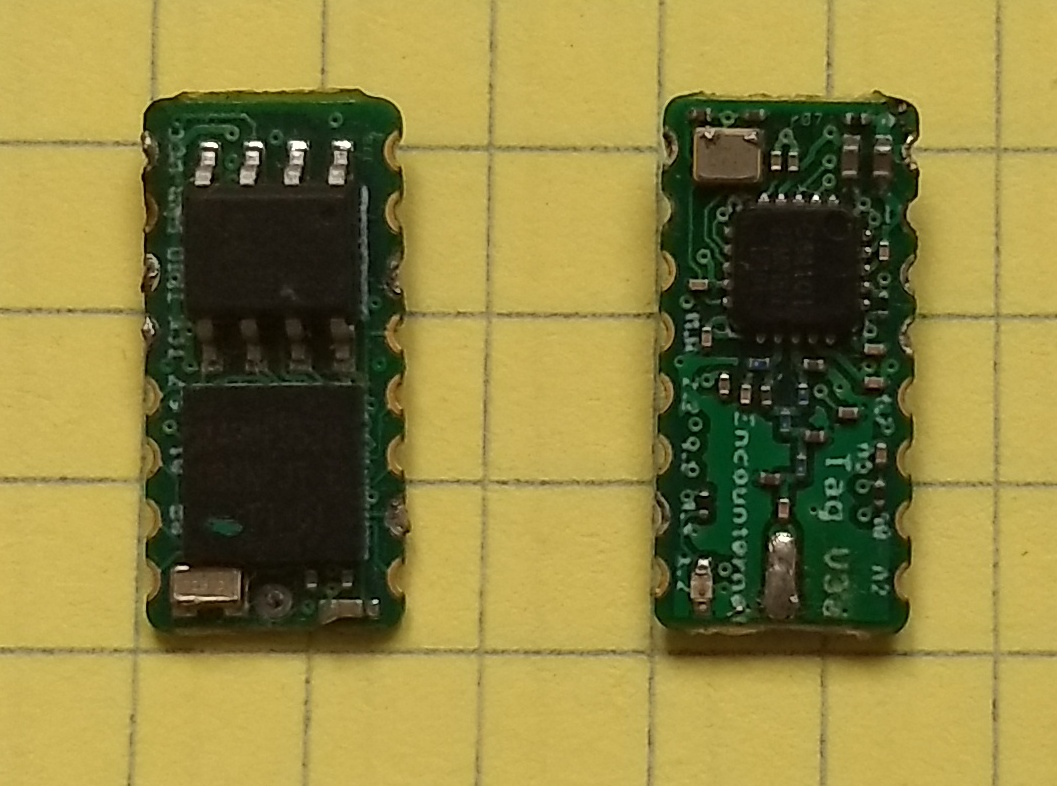
\includegraphics[width=3in]{figures/tag}
    \caption{Printed circuit boards for Encounternet tags~\protect\cite{Menhill2012NovelTelemetry}.
    Lines are 5mm apart. Complete tags require the addition of miniature batteries, whip antenna, and
    coating. The small batteries make effective protocols important.}
    \label{tags}
\end{figure}

Unfortunately, there is no robust encounter registration protocol 
for tag radios to transmit and receive packets efficiently.
The key challenge is the uncertain mobility and herd characteristics of wild 
animals. There is variability among species in their movement and 
interaction behavior. This issue adds a great deal of difficulties to
solve two challenging protocol-related problems. 
One problem is to minimize the power used for listening to other tags. 
All of the systems developed so far use low-power integrated
UHF transceivers, and the power consumed by these while receiving is 
comparable to the power that they use to transmit. 
The other protocol-related problem is interference. 
If many tags transmit simultaneously, receiving tags may fail
to reconstruct valid packets. Paradoxically, highly-efficient 
systems with good time synchronization and short activity
periods suffer more from this problem than less efficient systems 
in which the clocks of tags are not synchronized tightly
enough to transmit simultaneously. This is not a theoretical problem; 
many species of animals, including many species of
birds and bats, roost together, so encounters of tens or hundreds 
of individuals are not necessarily rare.

Our fundamental observation is that it is a waste of 
energy if an animal is not encountering with others
while still keeps the tag working frequently.
Thus it is reasonable for a tag to
increase the working frequency of its radio when 
encounter happens; otherwise it keeps
the radio in a low-power mode. 
To handle this issue while taking the uncertain mobility of animals into account, 
the dominant strategy in this paper is to design a mechanism
to identify the existence of an encounter in real-time. 

% The  strategy to address this issue appears to be duty-cycling the 
% receiver~\cite{Zhang2017Performance}, so that it is
% off most of the time. Synchronizing the timing of the activity periods 
% of all tags can minimize total receive energy
% while maximizing that transmissions will be received. 

% If tags do not synchronize their activity periods, many transmissions
% at close proximity may go unnoticed; this is not an unreasonable solution 
% if encounters are long. Another emerging approach
% to the receive-power problem is based on so-called {\em wake-up receivers}, 
% specialized nano-power sub-receivers whose only
% job is to wake up the main receiver when a strong packet is received. 
% These have not been used in Ecology research so we
% exclude them from most of the discussion; we do comment on 
% them in Section~\ref{sec:related-work}.

In this paper, we propose a robust protocol for encounter registration, 
addressing these problems mentioned above systematically and
methodically. In our protocol, we design two stages for the tags, 
namely detecting stage and connecting stage.
In the detecting stage, a tag works a fraction of time in order to save energy,
and transmits a beacon periodically to detect whether an encounter is happening at the moment.
When detected an acknowledgement, the tag switches to the connecting stage and increases the 
transmission frequency in order to establish links with other tags. To deal with interference 
happening in the connecting stage,
a tag adaptively adjusts its transmitting probability: it increases the probability when 
the channel is detected idle and reduces the probability when interference is detected.  


The contributions of the paper are summarized as follows:
\begin{itemize}
\item[1)] We formulate the problem model and propose a robust protocol for encounter registration problem 
with theoretical analyses. 
\item[2)] We conduct experiments and extensive simulations. Our evaluation results show that, 
compared to baseline methods, our protocol achieves lower latency, higher encounter 
registration rate and better scalability.
\item[3)] We present explicit animal models of mobility and evaluation results show that,
compared to baseline methods, our protocol has better performance, regarding three species
and three encounter cases.
\end{itemize}

%% Remaining structure
The remainder of the paper is organized as follows. 
The next section highlights the related works.
Section~\ref{sectionmodel} presents the system model and basic definitions.
We present the concrete protocol design
in Section~\ref{sectionprotocol}. 
%  We analyze the performance of our protocol in Section~\ref{sectionanalysis}. 
We carry out experiments for model validation in Section~\ref{experiments}
and simulations for protocol validation in in Section~\ref{Simulations}.
The paper is concluded in Section~\ref{sectionconclusion}.


